The Clang Static Analyzer is a tool that performs additional checking on C, C++, and Objective C source code. The checks performed by the static analyzer are more thorough than the checks the compiler performs. They are also more costly in terms of time and required resources. The static analyzer has a set of checkers that check for certain bugs.\par

The tool performs a symbolic interpretation of the source code that looks at all the code paths through an application and derives constraints on the values used in the application from it. Symbolic interpretation is a common technique used in compilers, for example, to identify constant values. In the context of the static analyzer, the checkers are applied to the derived values.\par

For example, if the divisor of a division is 0, then the static analyzer warns about it. We can check this with the following example stored in the div.c file:\par

\begin{lstlisting}[caption={}]
int divbyzero(int a, int b) { return a / b; }

int bug() { return divbyzero(5, 0); }
\end{lstlisting}

The static analyzer will warn about a division by 0 in the example. However, when compiling, the file with the clang -Wall -c div.c command will show no warning.\par

There are two ways to invoke the static analyzer from the command line. The older tool is scan-build, which is included in LLVM and can be used for simple scenarios. The newer tool is CodeChecker, available at \url{https://github.com/Ericsson/codechecker/}. For checking a single file, the scan-build tool is the easier solution. You simply pass the compile command to the tool, and everything else is done automatically:\par

\begin{tcolorbox}[colback=white,colframe=black]
\$ scan-build clang -c div.c \\
scan-build: Using '/usr/local/llvm12/bin/clang-12' for static \\
analysis \\
div.c:2:12: warning: Division by zero [core.DivideZero] \\
\hspace*{0.5cm}return a / b; \\
\hspace*{1.3cm}$\sim\sim\hat{}\sim\sim$ \\
1 warning generated. \\
scan-build: Analysis run complete. \\
scan-build: 1 bug found. \\
scan-build: Run 'scan-view /tmp/scanbuild-2021-03-01-023401-8721-1' \\
to examine bug reports.
\end{tcolorbox}

The output on the screen already tells you that a problem was found, that is, the checker with the name core.DivideZero was triggered. But that is not all. You will find a complete report in HTML in the mentioned subdirectory of the /tmp directory. You can use the scan-view command to view the report or open the index.html file found in the subdirectory in your browser.\par

The first page of the report shows you a summary of the found bugs:\par

\hspace*{\fill} \par %插入空行
\begin{center}
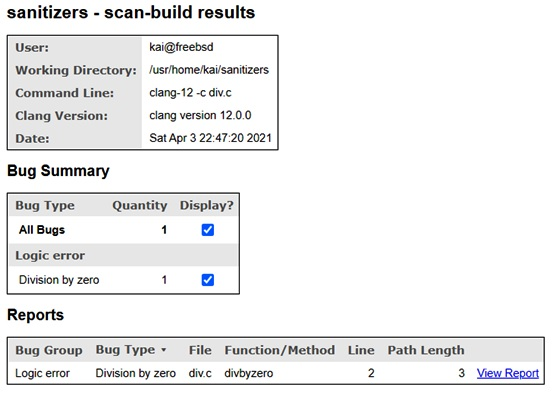
\includegraphics[width=1\textwidth]{content/3/chapter11/images/3.jpg}\\
Figure 11.3 – Summary page
\end{center}

For each found error, the summary page shows the type of the error, the location in the source, and the path length after which the analyzer finds the error. A link to a detailed report for the error is provided.\par

The following screenshot shows the detailed report for the error:\par


\hspace*{\fill} \par %插入空行
\begin{center}
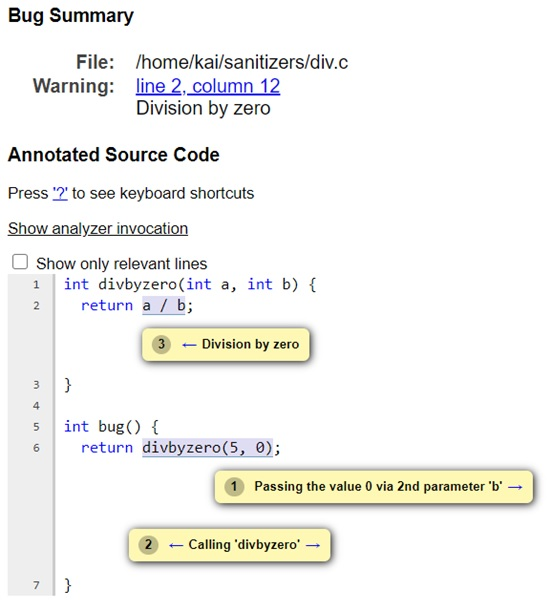
\includegraphics[width=0.8\textwidth]{content/3/chapter11/images/4.jpg}\\
Figure 11.4 – Detailed report
\end{center}

With the detailed report, you are able to verify the error by following the numbered bubbles. In our simple example, it shows in three steps how passing 0 as a parameter value leads to a division by zero error.\par
 
Verification through a human is indeed required. If the derived constraints are not precise enough for a certain checker, then false positives are possible, that is, an error is reported for perfectly fine code. Based on the report, you can identify false positives.\par

You are not limited to the checkers that are provided with the tool. You can also add new checkers. The next section shows how to do this.\par


\hspace*{\fill} \par %插入空行
\textbf{Adding a new checker to the Clang Static Analyzer}

To add a new checker to the Clang Static Analyzer, you create a new subclass of the Checker class. The static analyzer tries all possible paths through the code. The analyzer engine generates events at certain points, for example, before a function call or after a function call. Your class has to provide callbacks for these events if you need to handle them. The Checker class and the registrations for the events are provided in the clang/include/clang/StaticAnalyzer/Core/Checker.h header file.\par

Usually, a checker needs to track some symbols. But the checker can't manage the state, because it does not know which code path the analyzer engine currently tries. Therefore, the tracked state must be registered with the engine, and can only be changed using a ProgramStateRef instance.\par

Many libraries provide functions that must be used in pairs. For example, the C standard library provides the malloc() and free() functions. The memory allocated by the malloc() function must be freed exactly one time by the free() function. Not calling the free() function, or calling it several times, is a programming error. There are many more instances of this coding pattern, and the static analyzer provides checkers for some of them.\par

The iconv library provides functions to convert text from one encoding to another, for example, from Latin-1 encoding to UTF-16 encoding. To perform the conversion, the implementation needs to allocate memory. To transparently manage the internal resources, the iconv library provides the iconv\underline{~}open() and iconv\underline{~}close() functions, which must be used in pairs. You implement a checker to check for this.\par

To detect the errors, the checker needs to track the descriptor returned from the iconv\underline{~}open() function. The analyzer engine returns a SymbolRef instance for the return value of the iconv\underline{~}open() function. We associate this symbol with a state to reflect whether iconv\underline{~}close() was called or not. For the state, we create the IconvState class, which encapsulates a bool value.\par

The new IconvChecker class needs to handle four events:\par

\begin{itemize}
\item PostCall, which occurs after a function call. After the iconv\underline{~}open() function is called, we retrieve the symbol for the return value and remember it as being in an open state.

\item PreCall, which occurs before a function call. Before the iconv\underline{~}close() function is called, we check whether the symbol for the descriptor is in an open state. If not, then the iconv\underline{~}close() function was already called for the descriptor, and we have detected a double call to the function.

\item DeadSymbols, which occurs when unused symbols are cleaned up. We check whether an unused symbol for a descriptor is still in an open state. If yes, then we have detected a missing call to iconv\underline{~}close(), which is a resource leak.

\item PointerEscape, which is called when the symbols can no longer be tracked by the analyzer. In this case, we remove the symbol from the state, because we can no longer reason whether the descriptor was closed or not.

\end{itemize}

The new checker is implemented inside the Clang project. Let's begin with adding the new checker to the collection of all checkers, which is the clang/include/clang/StaticAnalyzer/Checkers/Checkers.td file. Each checker is associated with packages. Our new checker is under development, and therefore it belongs in the alpha package. The iconv API is a POSIX-standardized API, so it also belongs in the unix package. Locate the UnixAlpha section in the Checkers.td file and add the following code to register the new IconvChecker:\par

\begin{lstlisting}[caption={}]
def IconvChecker : Checker<"Iconv">,
	HelpText<"Check handling of iconv functions">,
	Documentation<NotDocumented>;
\end{lstlisting}

This adds the new checker to the collection of known checkers, sets help text for the command-line option, and states that there is no documentation for this checker.\par

Next, we implement the checker in the clang/lib/StaticAnalyzer/Checkers/IconvChecker.cpp file:\par

\begin{enumerate}
\item For the implementation, we need to include several header files. The BuiltinCheckerRegistration.h file is required to register the checker. The Checker.h file provides the declaration of the Checker class and the callbacks for the events. The CallEvent.h file declares the class used for call events, and the CheckerContext.h file is required for the declaration of the CheckerContext class, which is the central class providing access to the state of the analyzer:
\begin{lstlisting}[caption={}]
#include "clang/StaticAnalyzer/Checkers/
BuiltinCheckerRegistration.h"
#include "clang/StaticAnalyzer/Core/Checker.h"
#include "clang/StaticAnalyzer/Core/
PathSensitive/CallEvent.h"
#include "clang/StaticAnalyzer/Core/PathSensitive/
CheckerContext.h"
\end{lstlisting}


\item To avoid typing the namespace names, we use the clang and ento namespaces:
\begin{lstlisting}[caption={}]
using namespace clang;
using namespace ento;
\end{lstlisting}

\item We associate a state with each symbol representing an iconv descriptor. The state can be open or closed, and we use a bool-type variable, with the true value for an open state. The state value is encapsulated in the IconvState struct. This struct is used with a FoldingSet data structure, which is a hash set that filters duplicate entries. To be usable with this data structure implementation, the Profile() method is added here, which sets the unique bits of this struct. We put the struct into an anonymous namespace, to avoid pollution of the global namespace:
\begin{lstlisting}[caption={}]
namespace {
struct IconvState {
	const bool IsOpen;
	public:
	IconvState(bool IsOpen) : IsOpen(IsOpen) {}
	bool isOpen() const { return IsOpen; }
	bool operator==(const IconvState &O) const {
		return IsOpen == O.IsOpen;
	}
	void Profile(llvm::FoldingSetNodeID &ID) const {
		ID.AddInteger(IsOpen);
	}
};
}
\end{lstlisting}

\item The IconvState struct represents the state of an iconv descriptor, which is represented by a symbol of the SymbolRef class. This is best done with a map, which has the symbol as the key and the state as the value. As explained earlier, the checker cannot hold the state. Instead, the state must be registered with the global program state, which is done with the REGISTER\underline{~}MAP\underline{~}WITH\underline{~}PROGRAMSTATE macro. This macro introduces the IconvStateMap name, which we use later to access the map:
\begin{lstlisting}[caption={}]
REGISTER_MAP_WITH_PROGRAMSTATE(IconvStateMap, SymbolRef,
							   IconvState)
\end{lstlisting}

\item We also implement the IconvChecker class in an anonymous namespace. The requested PostCall, PreCall, DeadSymbols, and PointerEscape events are template parameters to the Checker base class:
\begin{lstlisting}[caption={}]
namespace {
	class IconvChecker
		: public Checker<check::PostCall, check::PreCall,
						 check::DeadSymbols,
						 check::PointerEscape> {
\end{lstlisting}

\item The IconvChecker class only has fields of the CallDescription type, which are used to identify iconv\underline{~}open(), iconv(), and iconv\underline{~}close() function calls in the program:
\begin{lstlisting}[caption={}]
	CallDescription IconvOpenFn, IconvFn, IconvCloseFn;
\end{lstlisting}

\item The report() method generates an error report. The important parameters to the method are an array of symbols, the type of the bug, and a bug description. Inside the method, a bug report is created for each symbol, and the symbol is marked as the interesting one for the bug. If a source range is provided as a parameter, then this is also added to the report. Finally, the report is emitted:
\begin{lstlisting}[caption={}]
	void
	report(ArrayRef<SymbolRef> Syms, const BugType &Bug,
		   StringRef Desc, CheckerContext &C,
		   ExplodedNode *ErrNode,
		   Optional<SourceRange> Range = None) const {
		for (SymbolRef Sym : Syms) {
			auto R = std::make_unique
					<PathSensitiveBugReport>(
				Bug, Desc, ErrNode);
			R->markInteresting(Sym);
			if (Range)
				R->addRange(*Range);
			C.emitReport(std::move(R));
		}
	}
\end{lstlisting}

\item The constructor of the IconvChecker class only initializes the CallDescription fields using the name of the function:
\begin{lstlisting}[caption={}]
public:
	IconvChecker()
		: IconvOpenFn("iconv_open"), IconvFn("iconv"),
			IconvCloseFn("iconv_close", 1) {}
\end{lstlisting}

\item The checkPostCall() method is called after the analyzer has executed a function call. If the executed function is not a global C function and not named iconv\underline{~}open, then there is nothing to do:
\begin{lstlisting}[caption={}]
	void checkPostCall(const CallEvent &Call,
					   CheckerContext &C) const {
		if (!Call.isGlobalCFunction() ||
			!Call.isCalled(IconvOpenFn))
			return;
\end{lstlisting}

\item Otherwise, we try to get the return value of the function as a symbol. To store the symbol with the open state in the global program state, we need to get a ProgramStateRef instance from the CheckerContext instance. The state is immutable, so adding the symbol to the state results in a new state. The analyzer engine is informed about the new state with a call to the addTransition() method:
\begin{lstlisting}[caption={}]
	if (SymbolRef Handle =
				Call.getReturnValue().getAsSymbol()) {
			ProgramStateRef State = C.getState();
			State = State->set<IconvStateMap>(
				Handle, IconvState(true));
			C.addTransition(State);
		}
	}
\end{lstlisting}

\item The checkDeadSymbols() method is called to clean up unused symbols. We loop over all symbols we track and ask the SymbolReaper instance whether the current symbol is dead:\par
\begin{lstlisting}[caption={}]
	void checkDeadSymbols(SymbolReaper &SymReaper,
						  CheckerContext &C) const {
		ProgramStateRef State = C.getState();
		SmallVector<SymbolRef, 8> LeakedSyms;
		for (auto SymbolState :
				State->get<IconvStateMap>()) {
			SymbolRef Sym = SymbolState.first;
			IconvState &St = SymbolState.second;
			
			if (SymReaper.isDead(Sym)) {
\end{lstlisting}

\item If the symbol is dead, then we need to check the state. If the state is still open, then this is a potential resource leak. There is one exception: iconv\underline{~}open() returns -1 in the case of an error. If the analyzer is in a code path handling this error, then it is wrong to assume a resource leak, because the function call failed. We try to get the value of the symbol from the ConstraintManager instance, and we do not consider the symbol as a resource leak if this value is -1. We add a leaked symbol to a SmallVector instance, for generating the error report later. Finally, we remove the dead symbol from the program state:
\begin{lstlisting}[caption={}]
				if (St.isOpen()) {
					bool IsLeaked = true;
					if (const llvm::APSInt *Val =
						State->getConstraintManager()
							.getSymVal(State, Sym))
						IsLeaked = Val->getExtValue() != -1;
					if (IsLeaked)
						LeakedSyms.push_back(Sym);
				}
			
				State = State->remove<IconvStateMap>(Sym);
			}
		}
\end{lstlisting}

\item After the loop, we call the generateNonFatalErrorNode() method. This method transitions to the new program state, and returns an error node if there is not already an error node for this path. The LeakedSyms container holds the (possibly empty) list of leaked symbols, and we call the report() method to generate an error report:
\begin{lstlisting}[caption={}]
		if (ExplodedNode *N =
				C.generateNonFatalErrorNode(State)) {
			BugType LeakBugType(this, "Resource Leak",
								"iconv API Error", true);
			report(LeakedSyms, LeakBugType,
				   "Opened iconv descriptor not closed", C,
					N);
		}
	}
\end{lstlisting}

\item The checkPointerEscape() function is called when the analyzer detects a function call for which the parameters cannot be tracked. In such a case, we must assume that we do not know whether the iconv descriptor will be closed inside the function or not. The only exception is a call to the iconv() function, which does the conversion and is known to not call the iconv\underline{~}close() function. This finishes the implementation of the IconvChecker class:
\begin{lstlisting}[caption={}]
	ProgramStateRef
	checkPointerEscape(ProgramStateRef State,
						const InvalidatedSymbols &Escaped,
						const CallEvent *Call,
						PointerEscapeKind Kind) const {
		if (Kind == PSK_DirectEscapeOnCall &&
			Call->isCalled(IconvFn))
			return State;
		for (SymbolRef Sym : Escaped)
			State = State->remove<IconvStateMap>(Sym);
		return State;
	}
};
}
\end{lstlisting}

\item Lastly, the new checker needs to be registered at a CheckerManager
instance. The shouldRegisterIconvChecker() method returns true to indicate that IconvChecker should be registered by default, and the registerIconvChecker() method performs the registration. Both methods are called via the code generated from the Checkers.td file:
\begin{lstlisting}[caption={}]
void ento::registerIconvChecker(CheckerManager &Mgr) {
	Mgr.registerChecker<IconvChecker>();
}

bool ento::shouldRegisterIconvChecker(
const CheckerManager &Mgr) {
	return true;
}
\end{lstlisting}

\end{enumerate}

This finishes the implementation of the new checker. You just need to add the filename to the list of source filenames in the clang/lib/StaticAnalyzer/Checkers/CmakeLists.txt file:\par

\begin{tcolorbox}[colback=white,colframe=black]
add\underline{~}clang\underline{~}library(clangStaticAnalyzerCheckers \\
… \\
\hspace*{0.5cm}IconvChecker.cpp \\
…)
\end{tcolorbox}

To compile the new checker, you change to your build directory and run the ninja command:\par

\begin{tcolorbox}[colback=white,colframe=black]
\$ ninja
\end{tcolorbox}

You can test the new checker with the following source saved in the conv.c file, which has two calls to the iconv\underline{~}close() function:\par

\begin{lstlisting}[caption={}]
#include <iconv.h>

void doconv() {
	iconv_t id = iconv_open("Latin1", "UTF-16");
	iconv_close(id);
	iconv_close(id);
}
\end{lstlisting}

You learned how to extend the Clang Static Analyzer with your own checker. You can use this knowledge to either create new general checkers and contribute them to the community, or you can create checkers specifically built for your needs, to raise the quality of your product. \par

The static analyzer is built leveraging the Clang infrastructure, and the next section introduces you to how can build your own plugin extending Clang.\par















